\iffalse
\title{04-2023}
\author{EE24BTECH11055}
\section{integer}
\fi
%\begin{enumerate}[start = 16]
\item The sum of all four-digit numbers that can be formed using all the digits $2, 1, 2, 3$ is equal to \underline{\hspace{1 cm}}. 
\item In the figure, $\theta_1 + \theta_2 = \frac{\pi}{2}$ and $\sqrt{3}\brak{BE} = 4\brak{AB}$. If the area of $\triangle CAB$ is $2\sqrt{3} - 3 {\text{unit}}^2$, when $\frac{\theta_2}{\theta_1}$ is the largest, then the perimeter of $\triangle CED$ is equal to \underline{\hspace{1 cm}}. 
	\begin{center}
	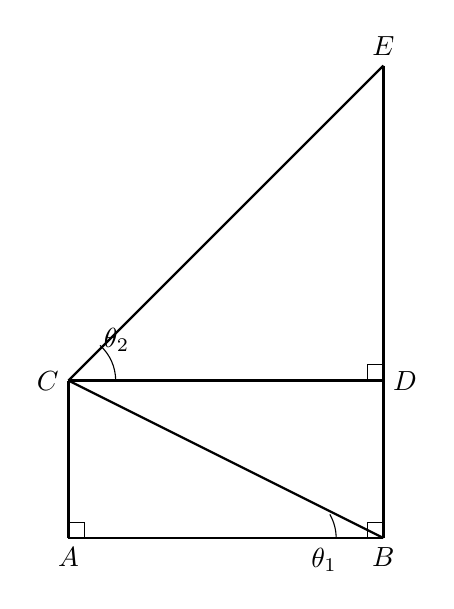
\begin{tikzpicture}
    \coordinate [label=below:$A$] (A) at (0,0);
    \coordinate [label=left:$C$] (C) at (0,2);
    \coordinate [label=below:$B$] (B) at (4,0);
    \coordinate [label=above:$E$] (E) at (4,6);
    \coordinate [label=right:$D$] (D) at (4,2);
    \draw [thick] (C) -- (E);
    \draw [thick] (E) -- (D);
    \draw [thick] (D) -- (C);
    \draw [thick] (A) -- (C);
    \draw [thick] (A) -- (B);
    \draw [thick] (B) -- (D);
    \draw [thick] (B) -- (C);
    \draw[draw] ([shift=(0:0.6cm)]C) arc[start angle=0, end angle=48, radius=0.6cm]; % Angle D-C-E
    \draw[draw] ([shift=(0:-0.6cm)]B) arc[start angle=0, end angle=30, radius=0.6cm]; % Angle C-B-A

    % Place the angle labels as nodes
    \node at ([shift=(40:0.8cm)]C) {$\theta_2$}; % Label for angle D--C--E
    \node at ([shift=(20:-0.8cm)]B) {$\theta_1$}; % Label for angle C--B--A
    %\pic [draw, "{$\theta_2$}", angle eccentricity=1.2] {angle = D--C--E};
    %\pic [draw, "{$\theta_1$}", angle eccentricity=1.2] {angle = C--B--A};
    %\tkzMarkRightAngle(E,D,C)
		%\tkzMarkRightAngle(C,A,B)
		%\tkzMarkRightAngle(D,B,A)
		\draw (D) -- ++(0,0.2) -- ++(-0.2,0) -- ++(0,-0.2); % Right angle at D for ∠EDC
    \draw (A) -- ++(0.2,0) -- ++(0,0.2) -- ++(-0.2,0); % Right angle at A for ∠CAB
    \draw (B) -- ++(0,0.2) -- ++(-0.2,0) -- ++(0,-0.2); % Right angle at B for ∠DBA
\end{tikzpicture}
	\end{center}
\item Let the tangent at any point $\vec{P}$ on a curve passing through the points $\brak{1,1}$ and $\brak{\frac{1}{10},100}$, intersect positive x-axis and y-axis at the points $\vec{A}$ and $\vec{B}$ respectively. If $PA : PB = 1 : k$ and $y=y\brak{x}$ is the solution of the differential equation $e^{\frac{dy}{dx}} = kx + \frac{k}{2}, y\brak{0} = k$, then $4y\brak{1} -\log e^3$ is equal to \underline{\hspace{1 cm}}. 
\item Suppose $a_1, a_2, 2, a_3, a_4$ be in an arithmetico-geometric progression. If the common ratio of the corresponding geometric progression is $2$ and the sum of all $5$ terms of the arithmetico-geometric progression is $\frac{49}{2}$, then $a_4$ is equal to \underline{\hspace{1 cm}}. 
\item If the area of the region $\cbrak{\brak{x,y} : \abs{x^2-2} \le x}$ is $A$, then $6A + 16\sqrt{2}$ is equal to \underline{\hspace{1 cm}}. 
\item Let the foot of perpendicular from the point $\vec{A} \brak{4,3,1}$ on the plane $P : x - y + 2z +3 = 0$ be $\vec{N}$. If $\vec{B}\brak{5,\alpha,\beta}, \alpha, \beta \in \mathbb{Z}$ is a point on plane $P$ such that the area of triangle $ABN$ is $3\sqrt{2}$, then $\alpha^2 + \beta^2 +\alpha\beta $ is equal to \underline{\hspace{1 cm}}. 
\item Let $S$ be the set of values of $\lambda$, for which the system of equations 
\begin{align*}
	6\lambda x - 3y + 3z &= 4\lambda^2,\\ 
	2x + 6\lambda y + 4z &= 1, \\
	3x + 2y + 3\lambda z &= \lambda 
\end{align*}
has no solution. Then $12 \sum_{\lambda \in S} |\lambda|$ is equal to \underline{\hspace{1 cm}}. 
\item If the domain of the function $f\brak{x} = \sec^{-1}\brak{\frac{2x}{5x+3}}$ is $[\alpha,\beta) \cup (\gamma,\delta]$, then $\abs{3\alpha +10\brak{\beta + \gamma} + 21\delta}$ is equal to \underline{\hspace{1 cm}}. 
\item Let the quadratic curve passing through the point $\brak{-1,0}$ and touching the line $y=x$ at $\brak{1,1}$ be $y=f\brak{x}$. Then the x-intercept of the normal to the curve at the point $\brak{\alpha,\alpha + 1}$ in the first quadrant is \underline{\hspace{1 cm}}.
\item Let the equations of two adjacent sides of a parallelogram $ABCD$ be $2x-3y=-23$ and $5x + 4y = 23$. If the equation of one of its diagonal $AC$ is $3x + 7y = 23$ and the distance of $A$ from the other diagonal is $d$, then $50d^2$ is equal to \underline{\hspace{1 cm}}. 
%\end{enumerate}

